% \fancypagestyle{plain}{%
%   \fancyhf{}%
%   \fancyhead[L]{\footnotesize\href{https://github.com/DSR3164/sdr/tree/v2}{github.com/DSR3164/sdr/tree/v2}}%
%   \fancyhead[R]{\hypersetup{hidelinks}\qrcode[height=1.4cm]{https://github.com/DSR3164/sdr/tree/v2}}
%   \fancyfoot[C]{\thepage}
% }

\chapter*{\practicetitle} %Принципы работы Soapy SDR и работа с Adalm Pluto. Формирование и передача сигналов произвольной формы
\textbf{Цель работы:} Получить практическое понимание работы SoapySDR и интерфейсов управления Adalm Pluto, а также освоить формирование и передачу произвольных I/Q-сигналов.
\addcontentsline{toc}{section}{\MakeUppercase{Цель работы}}

\sect{Краткие теоретические сведения}
ADALM-PLUTO использует 12-битный ЦАП/АЦП, поэтому каждый из компонентов I и Q может принимать значения от $-2^{11}$ до $2^{11}-1$, то есть от -2048 до 2047.
Для их хранения в C++ удобнее использовать тип \texttt{int16\_t}, так как меньшие типы не вмещают весь диапазон.
В этом случае один комплексный семпл (I+Q) занимает 4 байта.

\begin{figure}[H]
  \centering
  \includegraphics[height=1\textwidth, keepaspectratio]{images/\practicenumber/sample_struct}
  \caption{Структура сэмпла}
\end{figure}

\newpage
\sect{Ход работы}
Для формирования сигнала произвольной формы необходимо правильно заполнять буфер семплов.

\begin{figure}[H]
  \centering
  \includegraphics[height=1\textwidth, keepaspectratio]{images/\practicenumber/rect_signal}
  \caption{Пример сигнала из буфера заполенного \texttt{1500 << 4}}
\end{figure}

Я попробовал следующие варианты:

\begin{itemize}
  \item Заполнение буфера значениями \texttt{1500 << 4} и отправка 3 раза
  \begin{figure}[H]
    \centering
    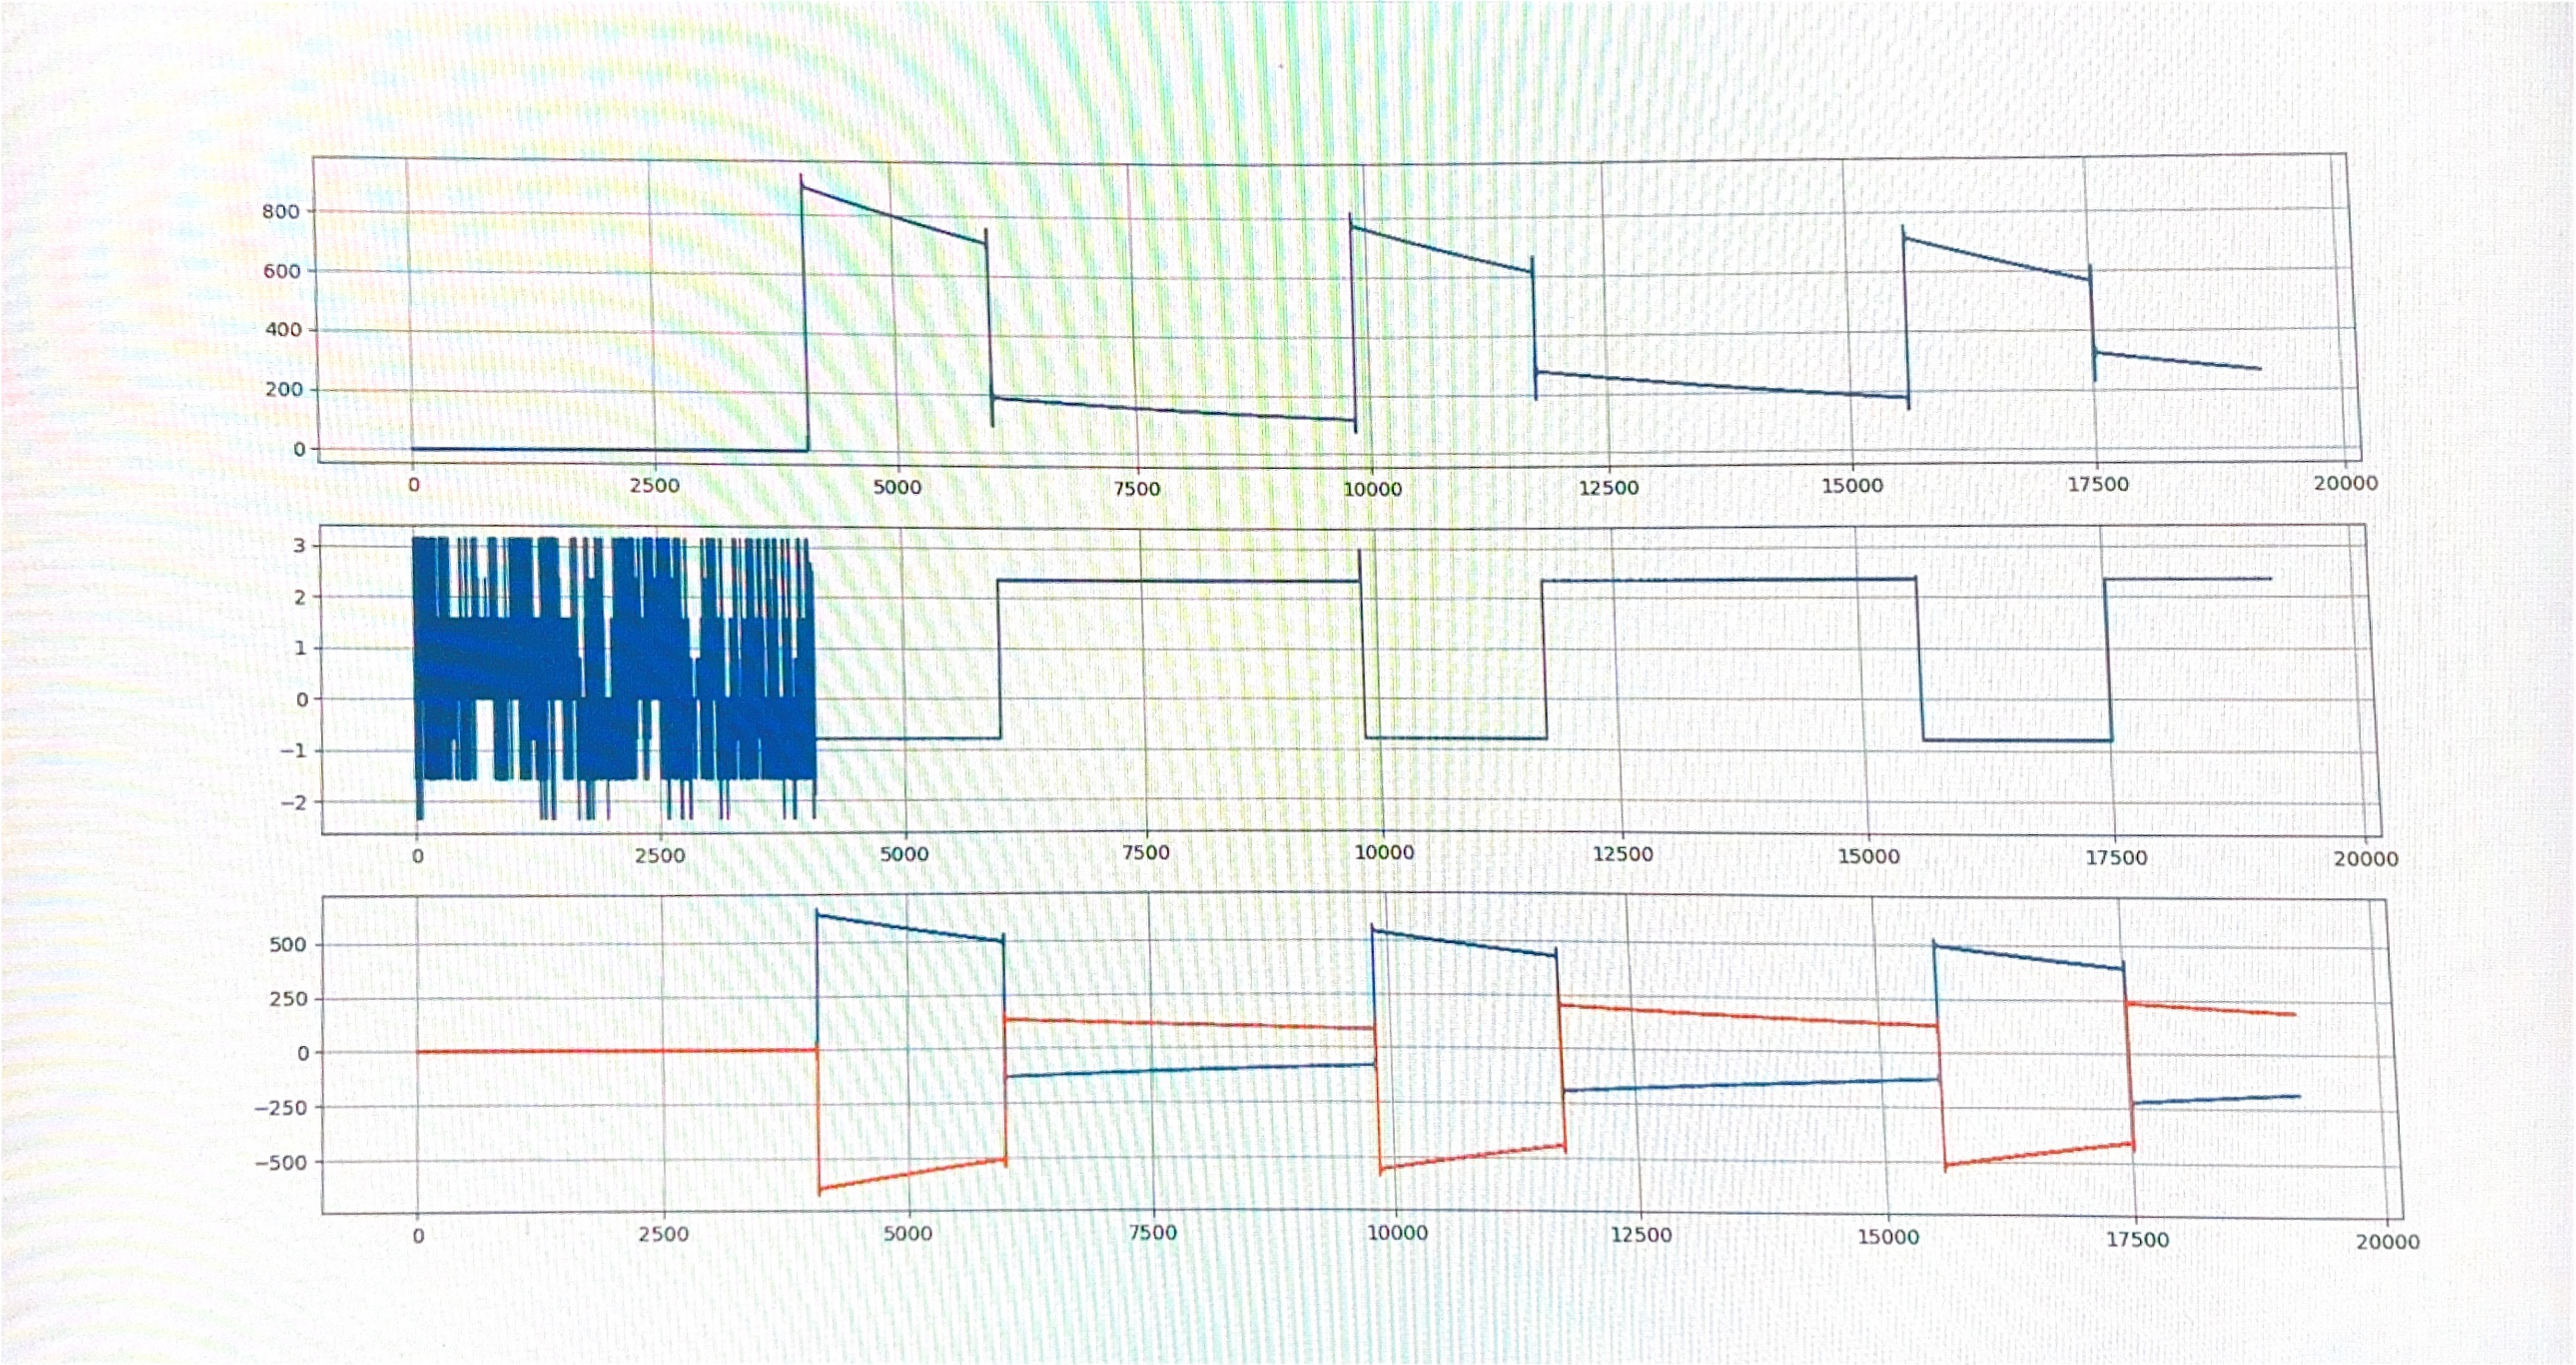
\includegraphics[height=1\textwidth, keepaspectratio]{images/\practicenumber/3_buff.jpg}
    \caption{Пример сигнала из буфера заполенного \texttt{1500 << 4}}
  \end{figure}
  \item Заполнение буфера значением \texttt{(2047 - i) << 4} для I и Q и отправка 50 раз
\end{itemize}

\begin{figure}[H]
  \centering
  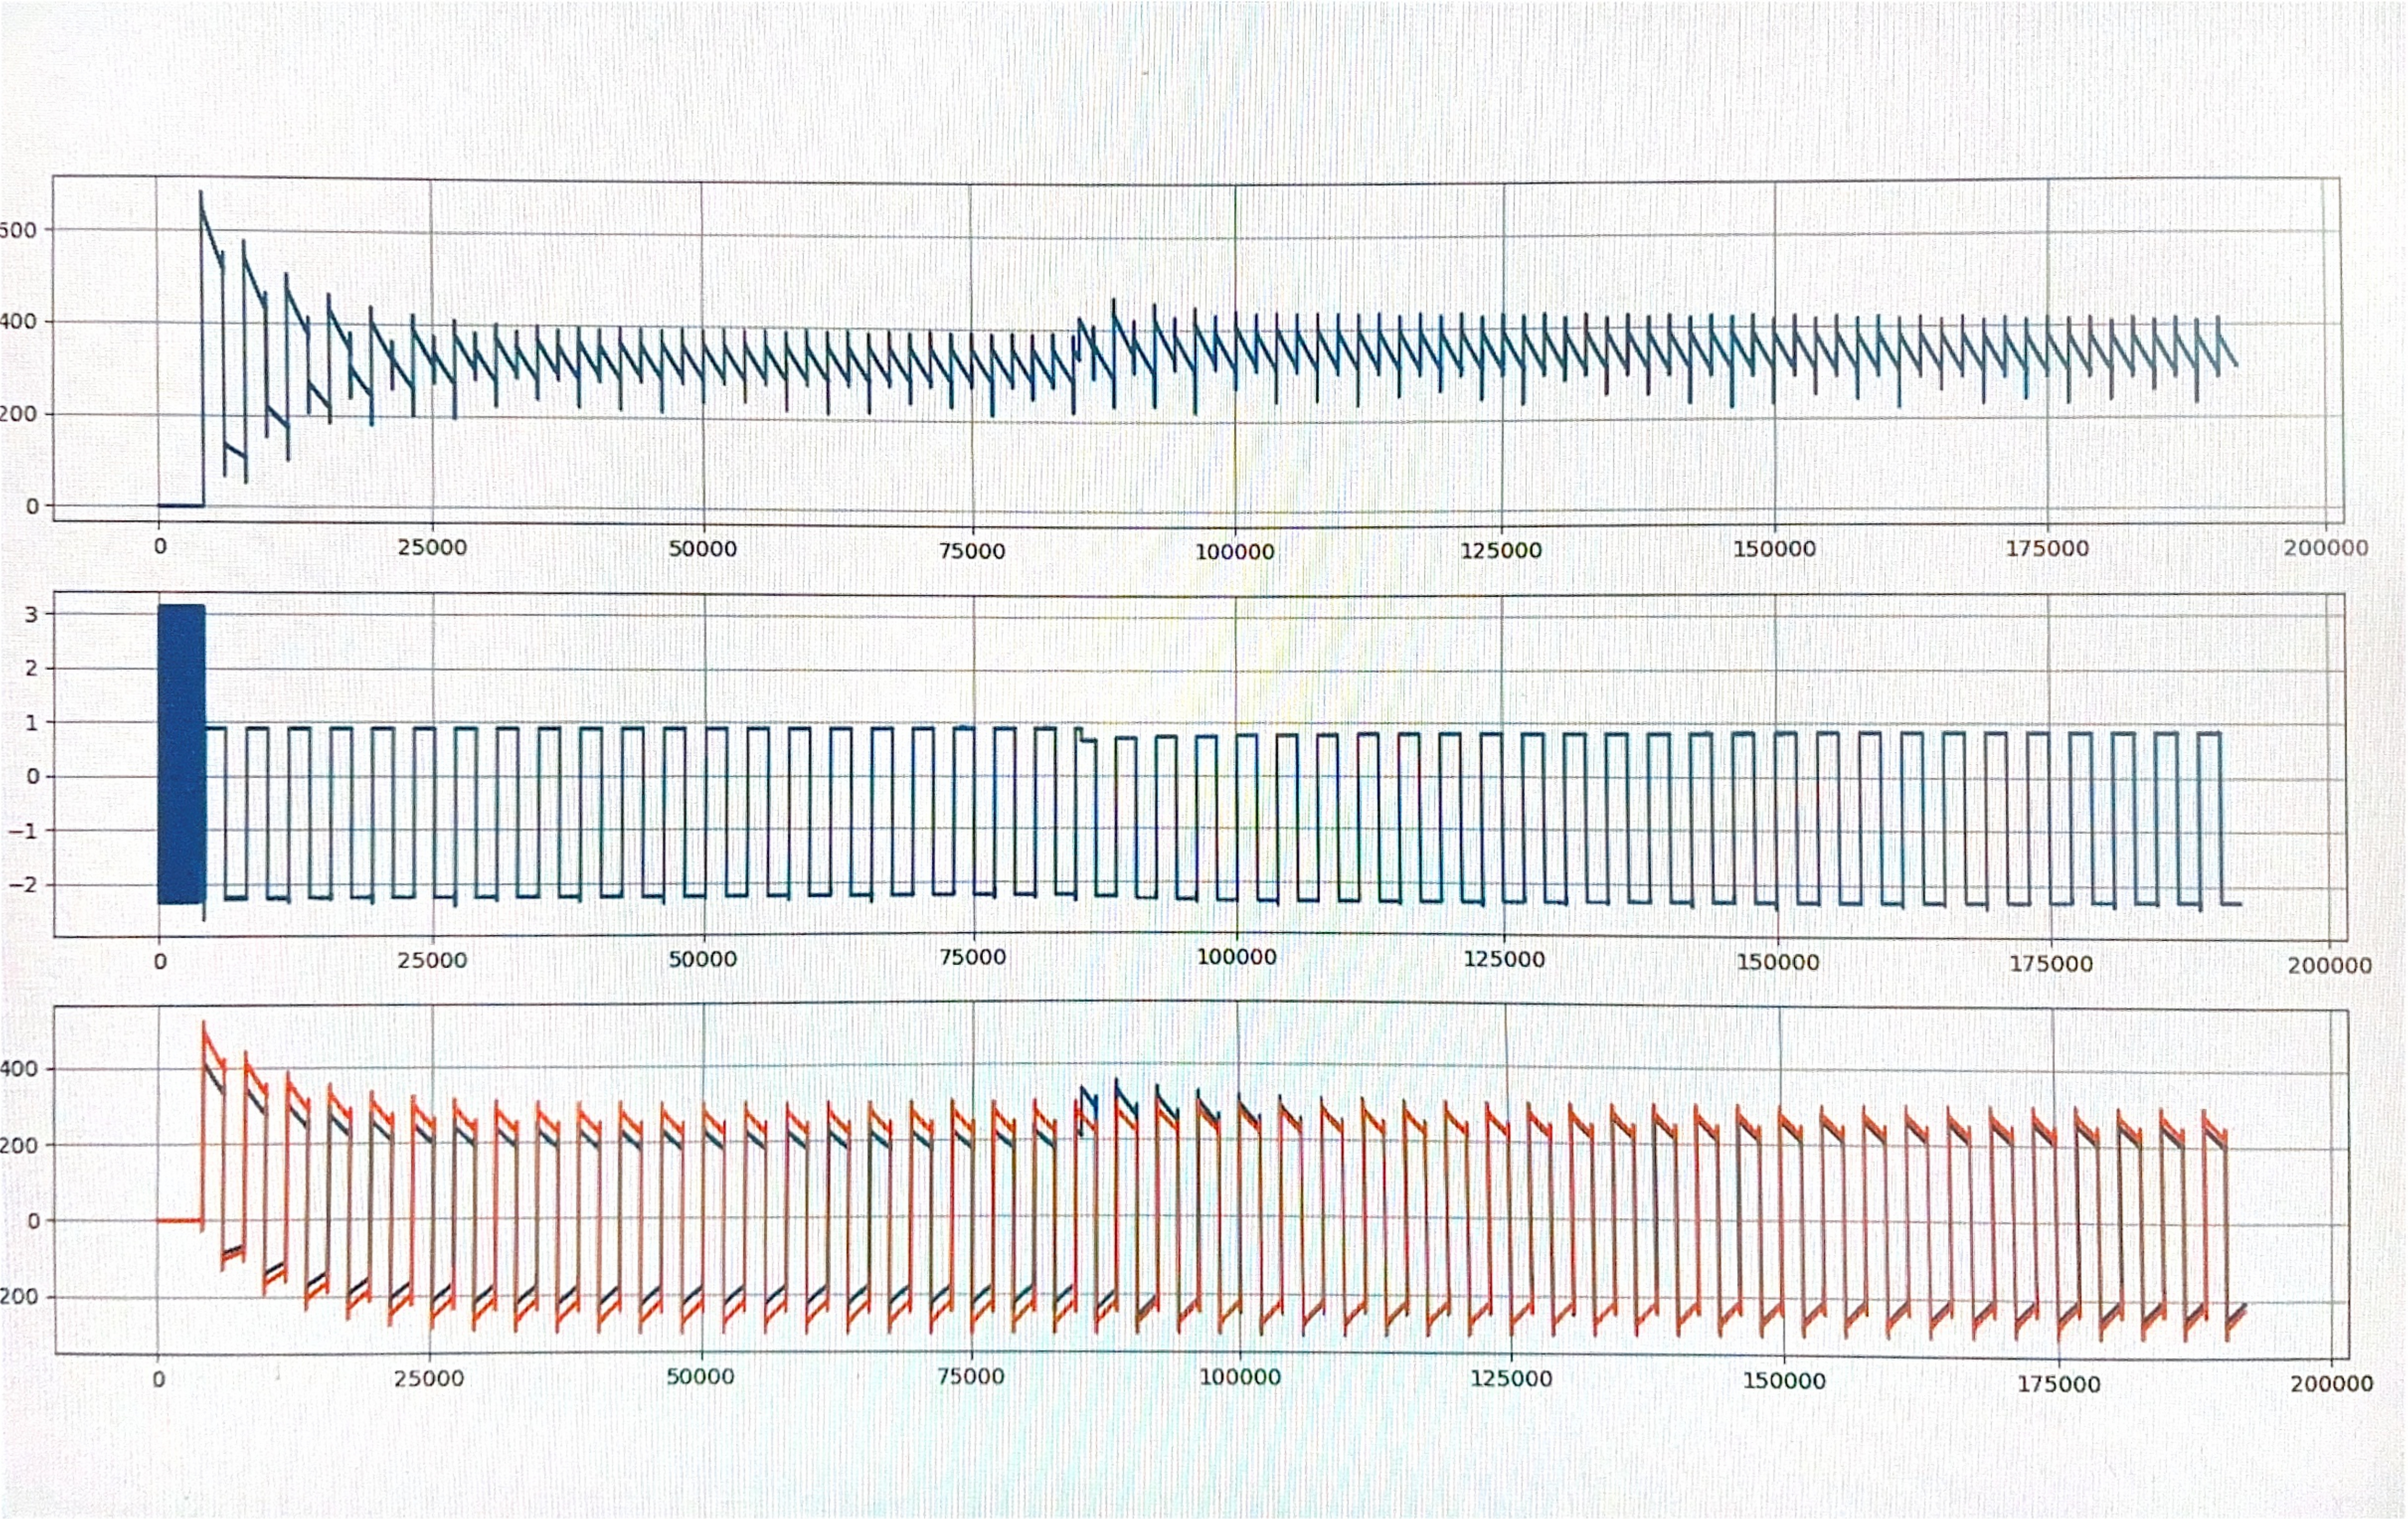
\includegraphics[height=1\textwidth, keepaspectratio]{images/\practicenumber/blade.jpg}
  \caption{Пример сигнала в форме пилы}
\end{figure}

\sect{Вывод}
Работа дала практическое понимание того, как через SoapySDR и интерфейсы управления Pluto можно напрямую формировать и отправлять произвольные I/Q-сигналы. Появилось ясное представление о цепочке: генерация выборок $\rightarrow$ настройка устройства $\rightarrow$ передача. А значит, стало понятно, что качество и корректность радиосигнала полностью зависят от точности собственной цифровой обработки